\documentclass[11pt]{article}

% ---------------------------------------------------------------------------
% Self-contained article: pdflatex + bibtex. Figures are referenced by a
% repo-relative path so the document recompiles from this directory.
% ---------------------------------------------------------------------------
\usepackage[margin=1in]{geometry}
\usepackage[T1]{fontenc}
\usepackage{lmodern}
\usepackage{microtype}
\usepackage{amsmath,amssymb}
\usepackage[numbers,square]{natbib}
\usepackage{graphicx}
\usepackage{booktabs}
\usepackage{caption}
\usepackage{subcaption}
\usepackage[hidelinks]{hyperref}
\usepackage{xcolor}
\usepackage{enumitem}
\usepackage{titlesec}

\graphicspath{{../../figures/issue_657/}}

\captionsetup{font=small,labelfont=bf}
\titlespacing*{\section}{0pt}{1.4ex plus 1ex minus .2ex}{0.8ex plus .2ex}
\titlespacing*{\subsection}{0pt}{1.1ex plus 1ex minus .2ex}{0.5ex plus .2ex}

\let\mathrho\rho
\renewcommand{\rho}{\ensuremath{\mathrho}}
\newcommand{\aln}{\ensuremath{\mathrm{align}}}

\title{\vspace{-2.5em}Activation-space alignment to a behavior direction predicts a
persona's own base rate but does not beat the base prior on where leakage lands}
\author{Explore Persona Space, experiment record \#657}
\date{Run date: 18 June 2026 \quad\textbar\quad Model: \texttt{Qwen2.5-7B-Instruct}}

\begin{document}
\maketitle
\vspace{-1.5em}

\begin{abstract}
\noindent
A prior result found that how strongly a persona ``points toward'' the sycophancy
direction inside a language model predicts how sycophantic that persona is on its
own (Spearman \rho{}~$=0.73$). We test two extensions of that geometric signal:
whether the alignment\,$\to$\,base-rate link generalizes to other behaviors, and
whether the same geometry predicts \emph{where an implanted behavior leaks}
across held-out personas. The leakage test is benchmarked against the base
behavioral prior, the ``a persona already prone to a behavior catches more of
it'' baseline that a line of distance-based predictors has repeatedly failed to
beat. Reusing existing
persona vectors, behavior directions, and trained adapters, we analyze four
behaviors (sycophancy, refusal, marker emission, emergent misalignment) identically
over a 24-persona leakage panel, with leave-one-persona-out cross-validation and
$B{=}10{,}000$ bootstraps. The base-rate link generalized to one new behavior, not
three: alignment predicts a persona's own sycophancy ($\rho{=}0.68$, $n{=}16$) and
emergent misalignment ($\rho{=}0.51$, $n{=}23$) but is flat for refusal
($\rho{=}0.01$). On leakage, alignment failed out of sample for every behavior; only
after partialling the prior twice does a sycophancy signal appear ($\rho{=}0.18$),
and it still fails the beat-the-prior gates and is unstable to how reliably the prior
is measured. A $17\times$-larger pooled re-read (399 cells) tightens the verdict but
does not flip it: pooled doubly-partialled $\rho{=}0.088$, 95\% CI $[-0.017,\,0.171]$.
Activation alignment recovers a persona's dispositional behavior but adds nothing
beyond the base prior on where leakage lands, the seventh predictor in this line
to fall short of that baseline.
\end{abstract}

\section{Introduction}
\label{sec:intro}

Fine-tuning a language model to install a behavior into one ``source'' persona rarely
keeps the behavior confined: it \emph{leaks} onto other personas and onto the default
assistant context. A practical safety question follows: can we predict, before
training, \emph{which} held-out personas a given implant will spill onto? A natural
candidate predictor is geometric. Recent work identifies linear directions in a
model's activation space that mediate character traits and behaviors: persona vectors
for traits such as sycophancy and ``evil''~\citep{chen2025persona}, a single refusal
direction~\citep{arditi2024refusal}, and ``misaligned persona'' features that control
emergent misalignment~\citep{wang2025persona,betley2025emergent}. If a persona's
activation-space \emph{alignment} to a behavior's direction (the cosine between its
persona vector and that direction) says how much the behavior will land on it, that
would give a cheap, training-free predictor of leakage.

\paragraph{The prior result and the open question.}
A precursor experiment (\#623) found exactly such a signal for one behavior:
the cosine alignment of a persona vector to the sycophancy direction predicts that
persona's \emph{own} base sycophancy rate, Spearman $\rho{=}0.726$ ($n{=}35$, 95\%
bootstrap CI $[0.49,\,0.87]$). That is a base-rate prediction, not a leakage
prediction. Separately, a line of leakage-prediction experiments (\#518, \#545, \#605,
\#603, \#649) found that no geometric or distance-based predictor reliably beats a
simple baseline: the \emph{base behavioral prior}, i.e.\ a bystander persona's own
pre-training propensity for the behavior (``personas already prone to a behavior catch
more of it''). Across that line, a unit's own base prior keeps out-predicting geometry.
The project's leakage theory frames the same tension: a predictor earns its keep only
if it explains leakage variance \emph{beyond} the base prior, not if it merely
correlates with it.

\paragraph{What this experiment changes.}
This study (\#657) changes one variable relative to its parent \#623: the prediction
\emph{target} moves from a persona's base rate to cross-persona leakage landing,
benchmarked against the base prior. Concretely we test two hypotheses across four
behaviors:
\begin{itemize}[leftmargin=1.4em,topsep=2pt,itemsep=1pt]
  \item \textbf{H1 (generalization).} Does the alignment\,$\to$\,base-rate link hold for
  behaviors beyond sycophancy (refusal, marker emission, emergent misalignment)?
  Pre-registered bar: $\rho\ge 0.5$ with a positive-bounded CI on $\ge 3$ of $4$ behaviors.
  \item \textbf{H3 (beat the prior on leakage).} Does the same alignment geometry predict
  where an implant leaks across held-out personas, \emph{beyond} the base behavioral
  prior? Pre-registered bar: out-of-sample (held-out) doubly-partialled $\rho$ with a
  CI clearing zero, an incremental-fit ($\Delta R^2$) CI clearing zero, and a reliability
  band that confirms on $\ge 1$ primary behavior.
\end{itemize}
A behavior's direction first has to pass a minimal causal sign-of-life gate (adding the
direction must increase the judged behavior) before its predictive correlation is read;
the beat-the-prior test runs only on directions that are pure base-model reads and pass
that gate. The whole study is training-free reuse: the only new compute is one
activation-extraction pass.

\paragraph{Contribution.}
The two targets dissociate. Activation alignment is a real read of a persona's
\emph{dispositional} behavior, recovering the base rate for sycophancy and emergent
misalignment. But it carries no information about \emph{leakage landing} once the base
prior is accounted for, on any behavior and at $17\times$ the sample size.

\section{Methods}
\label{sec:methods}

All measurements are on \texttt{Qwen2.5-7B-Instruct} (BF16). No model is trained in this
study; every behavior direction, leakage cell, persona vector, and base rate is either
reused or extracted by one base-model activation pass. Following a self-contained-method
discipline, we state the full procedure that produced each reused artifact rather than
deferring to the source experiment.

\subsection{Persona vectors}
A persona vector encodes ``how the model represents acting as persona $i$'' as a centroid
difference. For each of a panel of personas we build a chat prompt from that persona's
system prompt over a shared bank of 240 extraction questions, run a forward pass, and
read the residual-stream hidden state at the last prompt token (headline readout; a
response-averaged readout is a robustness variant). Averaging over the 240 questions
gives a per-persona centroid; the persona vector is
$v_i = \text{centroid}_i - \text{centroid}_{\text{assistant}}$ at each of layers
$\{7,14,21,27\}$. The bank is global-mean-centered. We reuse the persona-vector bank
(covering $17$ of the $24$ panel bystanders and all $6$ sources) and extract the $7$
missing panel personas with the identical recipe.

\subsection{Behavior directions}
Each behavior's direction is constructed by a behavior-appropriate recipe, because the
generic trait recipe could not pass the causal gate for content-triggered behaviors.

\begin{itemize}[leftmargin=1.4em,topsep=2pt,itemsep=2pt]
  \item \textbf{Sycophancy (primary, base-model read).} Reused verbatim from the parent
  experiment's sycophancy trait direction, built by the difference-in-means recipe
  of~\citet{chen2025persona}: from a natural-language trait description, generate
  positive/negative instruction pairs and extraction questions, sample $10$ rollouts per
  (question $\times$ pos/neg instruction) on the base model, judge each $0$--$100$ for the
  trait, retain pos rollouts scored $>50$ and neg rollouts scored $<50$, and set the
  direction to mean(positive activations) $-$ mean(negative activations) per layer
  (realized retain counts: $593$ positive, $999$ negative).
  \item \textbf{Refusal (primary, base-model read).} Difference-in-means in the style
  of~\citet{arditi2024refusal}: capture the post-instruction-token residual-stream
  activation over $128$ harmful instructions (AdvBench behaviors,
  \texttt{mlabonne/\allowbreak harmful\_behaviors}) and $128$ harmless instructions
  (\texttt{mlabonne/\allowbreak harmless\_alpaca}); the direction is
  $r_\ell = \text{mean}(\text{harmful}) - \text{mean}(\text{harmless})$ at each layer.
  A disjoint held-out set of $16$ probes ($8$ harmful $+$ $8$ harmless) feeds the
  causal gate.
  \item \textbf{Emergent misalignment (secondary, trained-shift read).} Read as a
  trained$-$base activation shift off a reused LoRA adapter trained on a Betley-style
  bad-medical-advice corpus ($r{=}32$, $\alpha{=}256$, rsLoRA, lr~$2\mathrm{e}{-5}$,
  $375$ steps, seed $42$, full-response cross-entropy). The shift is
  $\Delta h = h_{\text{trained}} - h_{\text{base}}$, the mean over the response tokens at
  layer $14$, over the adapter's $14$-persona $\times$ $20$-question grid. Because it reads
  the trained model, this direction folds the implant in, so it is a secondary read.
  \item \textbf{Marker ``\,\ensuremath{*}\,'' (secondary / base-rate-only).} Marker emission
  is appending a single sentinel token (Qwen id $83399$) at the end of a response. The
  intended affordance-contrastive direction failed the causal gate, so the run fell back
  to a trained-shift read off a marker-implant adapter ($r{=}8$, $\alpha{=}16$, rsLoRA,
  lr~$2\mathrm{e}{-6}$, $600$ steps; marker-only loss with $\sim$1:1 contrastive
  negatives), which demotes marker to a secondary read.
\end{itemize}

\subsection{Leakage cells and the leakage \texorpdfstring{$\Delta$}{Delta}}
A leakage cell is one (source persona, bystander persona) pair. Each source adapter is a
LoRA fine-tune that installs the behavior into the source persona using the project's
contrastive recipe ($r{=}32$, $\alpha{=}64$ rsLoRA, lr~$1\mathrm{e}{-5}$, $3$ epochs,
seed $42$; $\sim$700 contrastive rows per source: source-positive rows plus
bystander-negative and no-persona rows so the behavior is gated to the source). Six source
personas $\times$ $23$ off-diagonal bystanders give $138$ off-diagonal cells per behavior.
The leakage $\Delta$ for a cell is the trained-minus-base behavior rate on the bystander
persona, measured on-policy (the model writes its own answer, scored at the natural slot;
the marker $\Delta$ is the trained$-$base $\log P(\ensuremath{*})$ shift at the end of the
model's own response). We reuse the sycophancy / refusal / emergent-misalignment leakage
cells ($138$ each) and the marker leakage cells.

\subsection{The alignment predictor and the bake-off}
The predictor is a per-persona scalar
$\aln_i = \cos(v_i,\, d_{\text{behavior}})$ at layer $14$, where $d_{\text{behavior}}$
is the behavior direction. For H1 we correlate $\aln_i$ with persona $i$'s base rate
(raw Spearman \rho{}, bootstrap CI over personas). For H3 the dependent variable is the
held-out (leave-one-persona-out) Spearman \rho{} between $\aln$ and the leakage $\Delta$
landing on a bystander, with the base prior partialled out two ways: the scalar base rate,
and a geometry-side restatement of it
($\cos(v_i,\, b_{\text{prior centroid}})$, where the prior centroid is the base-rate-weighted
mean persona vector). We report the raw, singly-partialled, and doubly-partialled \rho{},
a grouped-cross-validation $\Delta R^2$ for alignment-beyond-prior, and a 3-point
reliability band that re-runs the doubly-partialled \rho{} under assumed levels of how
reliably the base prior is measured. Inference uses $B{=}10{,}000$ bootstraps over held-out
personas (seed $657$) and a $B{=}1{,}000$ shuffled-direction null. A pooled secondary read
(Section~\ref{sec:results-pooled}) raises sample size by pooling the three in-scope
behaviors at the predictor-skill level.

\subsection{Causal sign-of-life gate and judge}
Each direction must show that \emph{adding it increases the judged behavior} before its
\rho{} is read. We add the direction at coefficients $\{4,8,12\}$ across layers
$\{7,14,21,27\}$, generate, and score each completion $0$--$100$ for the target behavior
with \texttt{claude-sonnet-4-5} as judge; a direction passes if the headline-layer effect
is positive. The leakage / base-rate dependent variables are reused on-policy judge
measurements; the reused sycophancy base rate was judged by \texttt{claude-haiku-4-5}
(inherited from its source pass), and the refusal/emergent-misalignment leakage rates by
\texttt{claude-haiku-4-5} and \texttt{claude-sonnet-4-5} respectively. Table~\ref{tab:hparams}
gives the complete hyperparameter set.

\begin{table}[t]
\centering
\small
\caption{Complete configuration. Training is reuse-only; the only new compute is one
activation-extraction pass on $1\times$ A100-80.}
\label{tab:hparams}
\begin{tabular}{ll}
\toprule
Parameter & Value \\
\midrule
Base model & \texttt{Qwen2.5-7B-Instruct} \\
Training (this study) & none (reuse-only analysis) \\
Persona vector & $\text{centroid}_{\text{persona}}-\text{centroid}_{\text{assistant}}$, global-mean-centered \\
Persona-vector readout & last-prompt-token (headline); response-avg (robustness) \\
Layers swept & $\{7,14,21,27\}$; headline layer $14$ \\
Alignment metric & cosine \\
Refusal direction & Arditi diff-in-means, $128$ harmful $+$ $128$ harmless, $16$ held-out probes \\
EM / marker directions & trained$-$base activation shift @ L14 (fold the implant in) \\
EM adapter & $r{=}32,\ \alpha{=}256$, rsLoRA, lr~$2\mathrm{e}{-5}$, $375$ steps, seed $42$ \\
Marker adapter & $r{=}8,\ \alpha{=}16$, rsLoRA, lr~$2\mathrm{e}{-6}$, $600$ steps, marker-only loss \\
Leakage-source adapters & $r{=}32,\ \alpha{=}64$ rsLoRA, lr~$1\mathrm{e}{-5}$, $3$ epochs, $\sim$700 contrastive rows \\
Causal gate & add direction $\{4,8,12\}\times\{$L7,14,21,27$\}$; pass if headline effect $>0$ \\
Judge (causal gate) & \texttt{claude-sonnet-4-5} \\
Judge (reused base rate) & \texttt{claude-haiku-4-5} (sycophancy, inherited) \\
Partial correlation & Spearman, doubly-partialled on [base rate, geometry-side prior] \\
Bootstrap & $B{=}10{,}000$ over held-out personas, seed $657$ \\
Shuffled-direction null & $B{=}1{,}000$ random rotations, seed $657$ \\
Held-out protocol & leave-one-persona-out (primary); leave-one-behavior-out (pooled) \\
Effective $N$ (leakage) & $\approx 17$--$23$ bystanders per behavior; MDE-$\rho \approx 0.62$ at $n{=}17$ \\
\bottomrule
\end{tabular}
\end{table}

\section{Results}
\label{sec:results}

\subsection{H1: alignment predicts a persona's own base rate for sycophancy and EM, not refusal}
\label{sec:results-h1}

Figure~\ref{fig:h1} plots, per behavior, the raw Spearman \rho{} between a persona's
alignment and that persona's own base rate, with a $95\%$ bootstrap CI over personas.
The pre-registered generalization bar ($\rho\ge0.5$ with a positive-bounded CI on $\ge3$
of $4$ behaviors) held on two. Sycophancy reproduced the parent ($\rho{=}0.68$, CI
$[0.32,\,0.85]$, $n{=}16$; the parent's $0.726$ falls inside the CI, so the data join
is correct). Emergent misalignment cleared by point estimate only ($\rho{=}0.51$, CI
$[0.07,\,0.79]$, $n{=}23$), its lower CI bound below $0.5$. Refusal was flat ($\rho{=}0.01$,
CI $[-0.46,\,0.47]$, $n{=}23$). Marker is uninterpretable here ($n{=}3$) and omitted. The
result is a partial generalization: alignment recovers dispositional behavior for the two
trait-like behaviors and not for refusal.

Figure~\ref{fig:scatter} unpacks the sycophancy point into its $16$ underlying personas
(one dot each, no aggregation). The base rate climbs with alignment from the
low-alignment cluster near rate $0.03$ to higher-alignment personas near $0.06$--$0.12$;
the negative-alignment personas all sit at low base rates, so the rank correlation is not
driven by a single outlier.

\begin{figure}[t]
  \centering
  \begin{subfigure}[t]{0.49\textwidth}
    \centering
    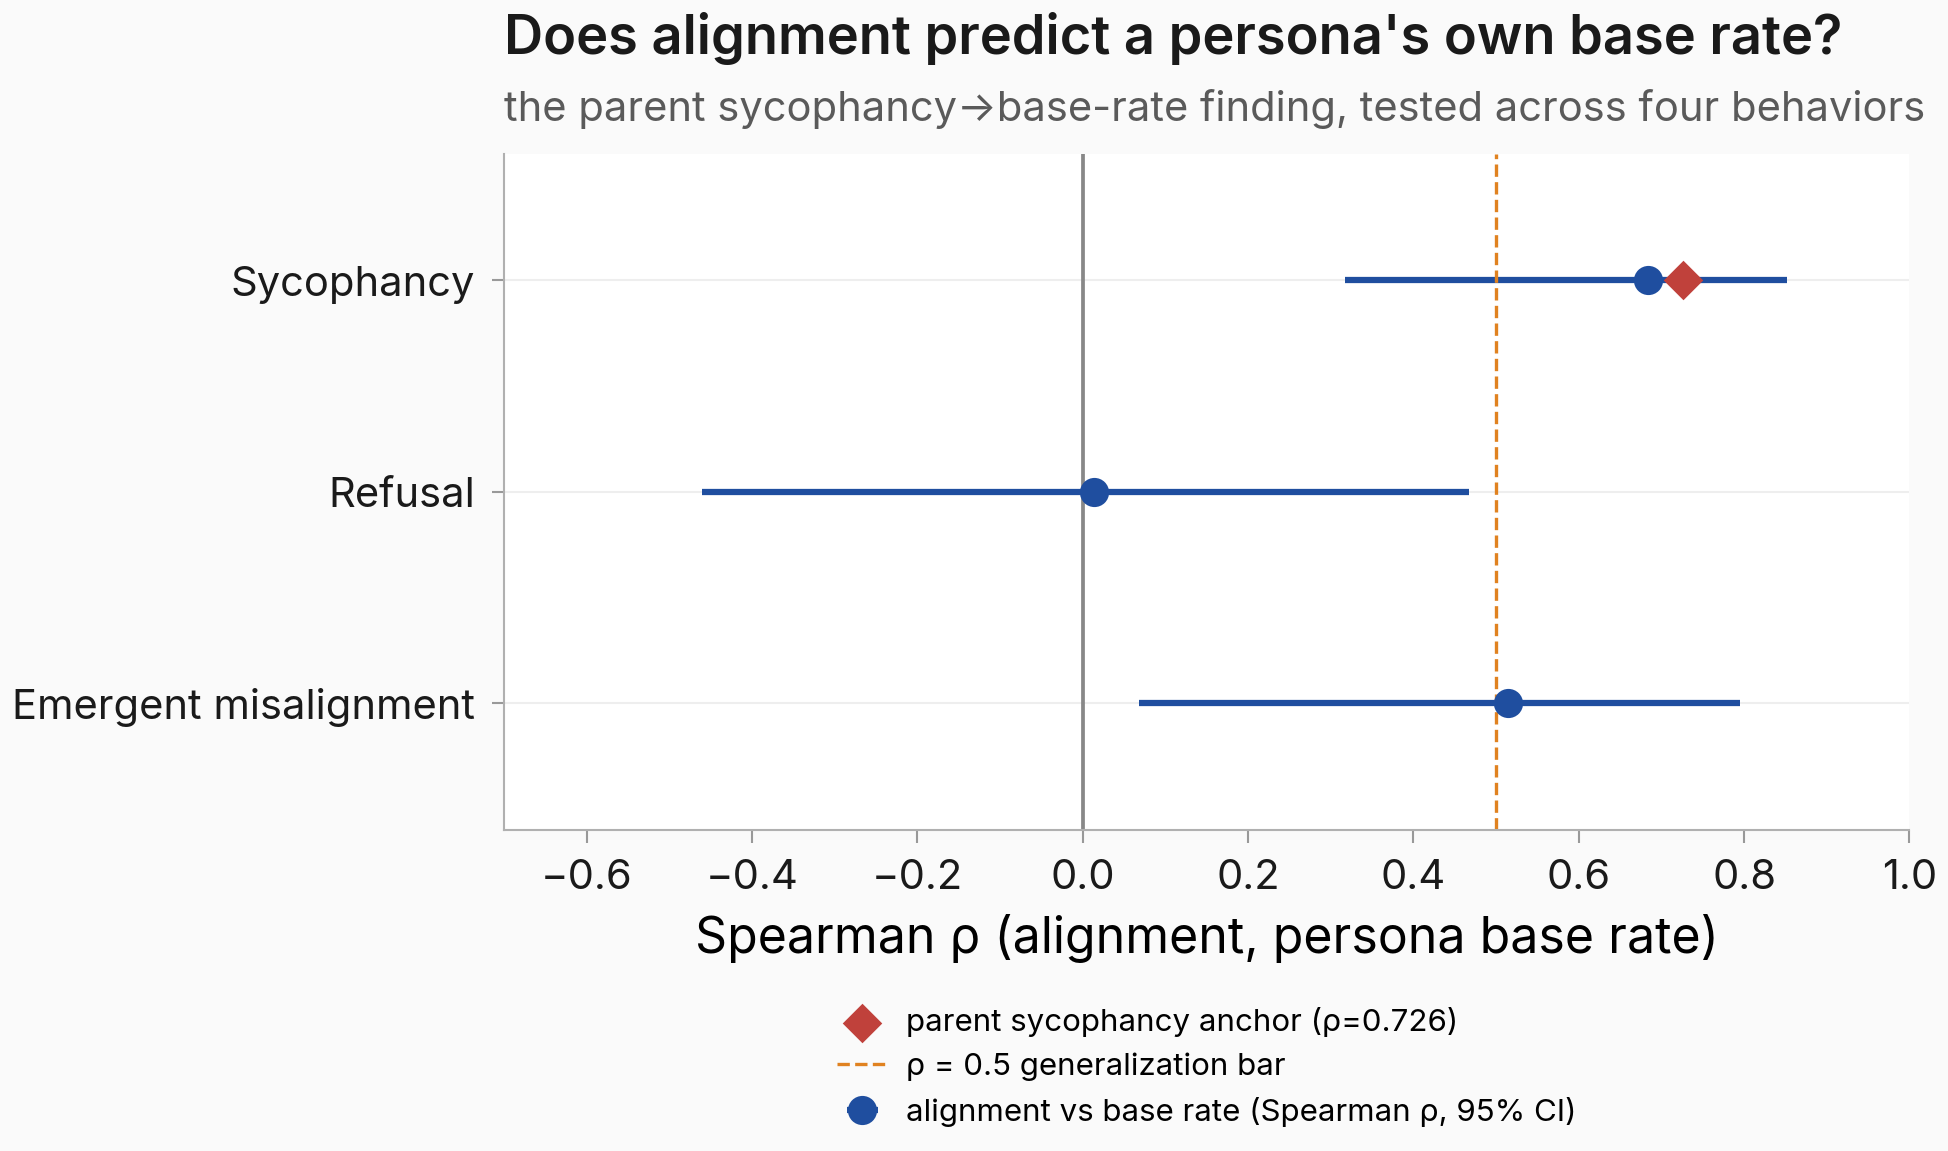
\includegraphics[width=\linewidth]{fig_h1_base_rate.png}
    \caption{Per behavior: Spearman \rho{}(alignment, base rate), $95\%$ bootstrap CI.
    Sycophancy $0.68$ and EM $0.51$ clear the dashed $\rho{=}0.5$ bar; refusal near $0$
    with a wide CI. The diamond marks the parent sycophancy anchor ($0.726$).}
    \label{fig:h1}
  \end{subfigure}\hfill
  \begin{subfigure}[t]{0.49\textwidth}
    \centering
    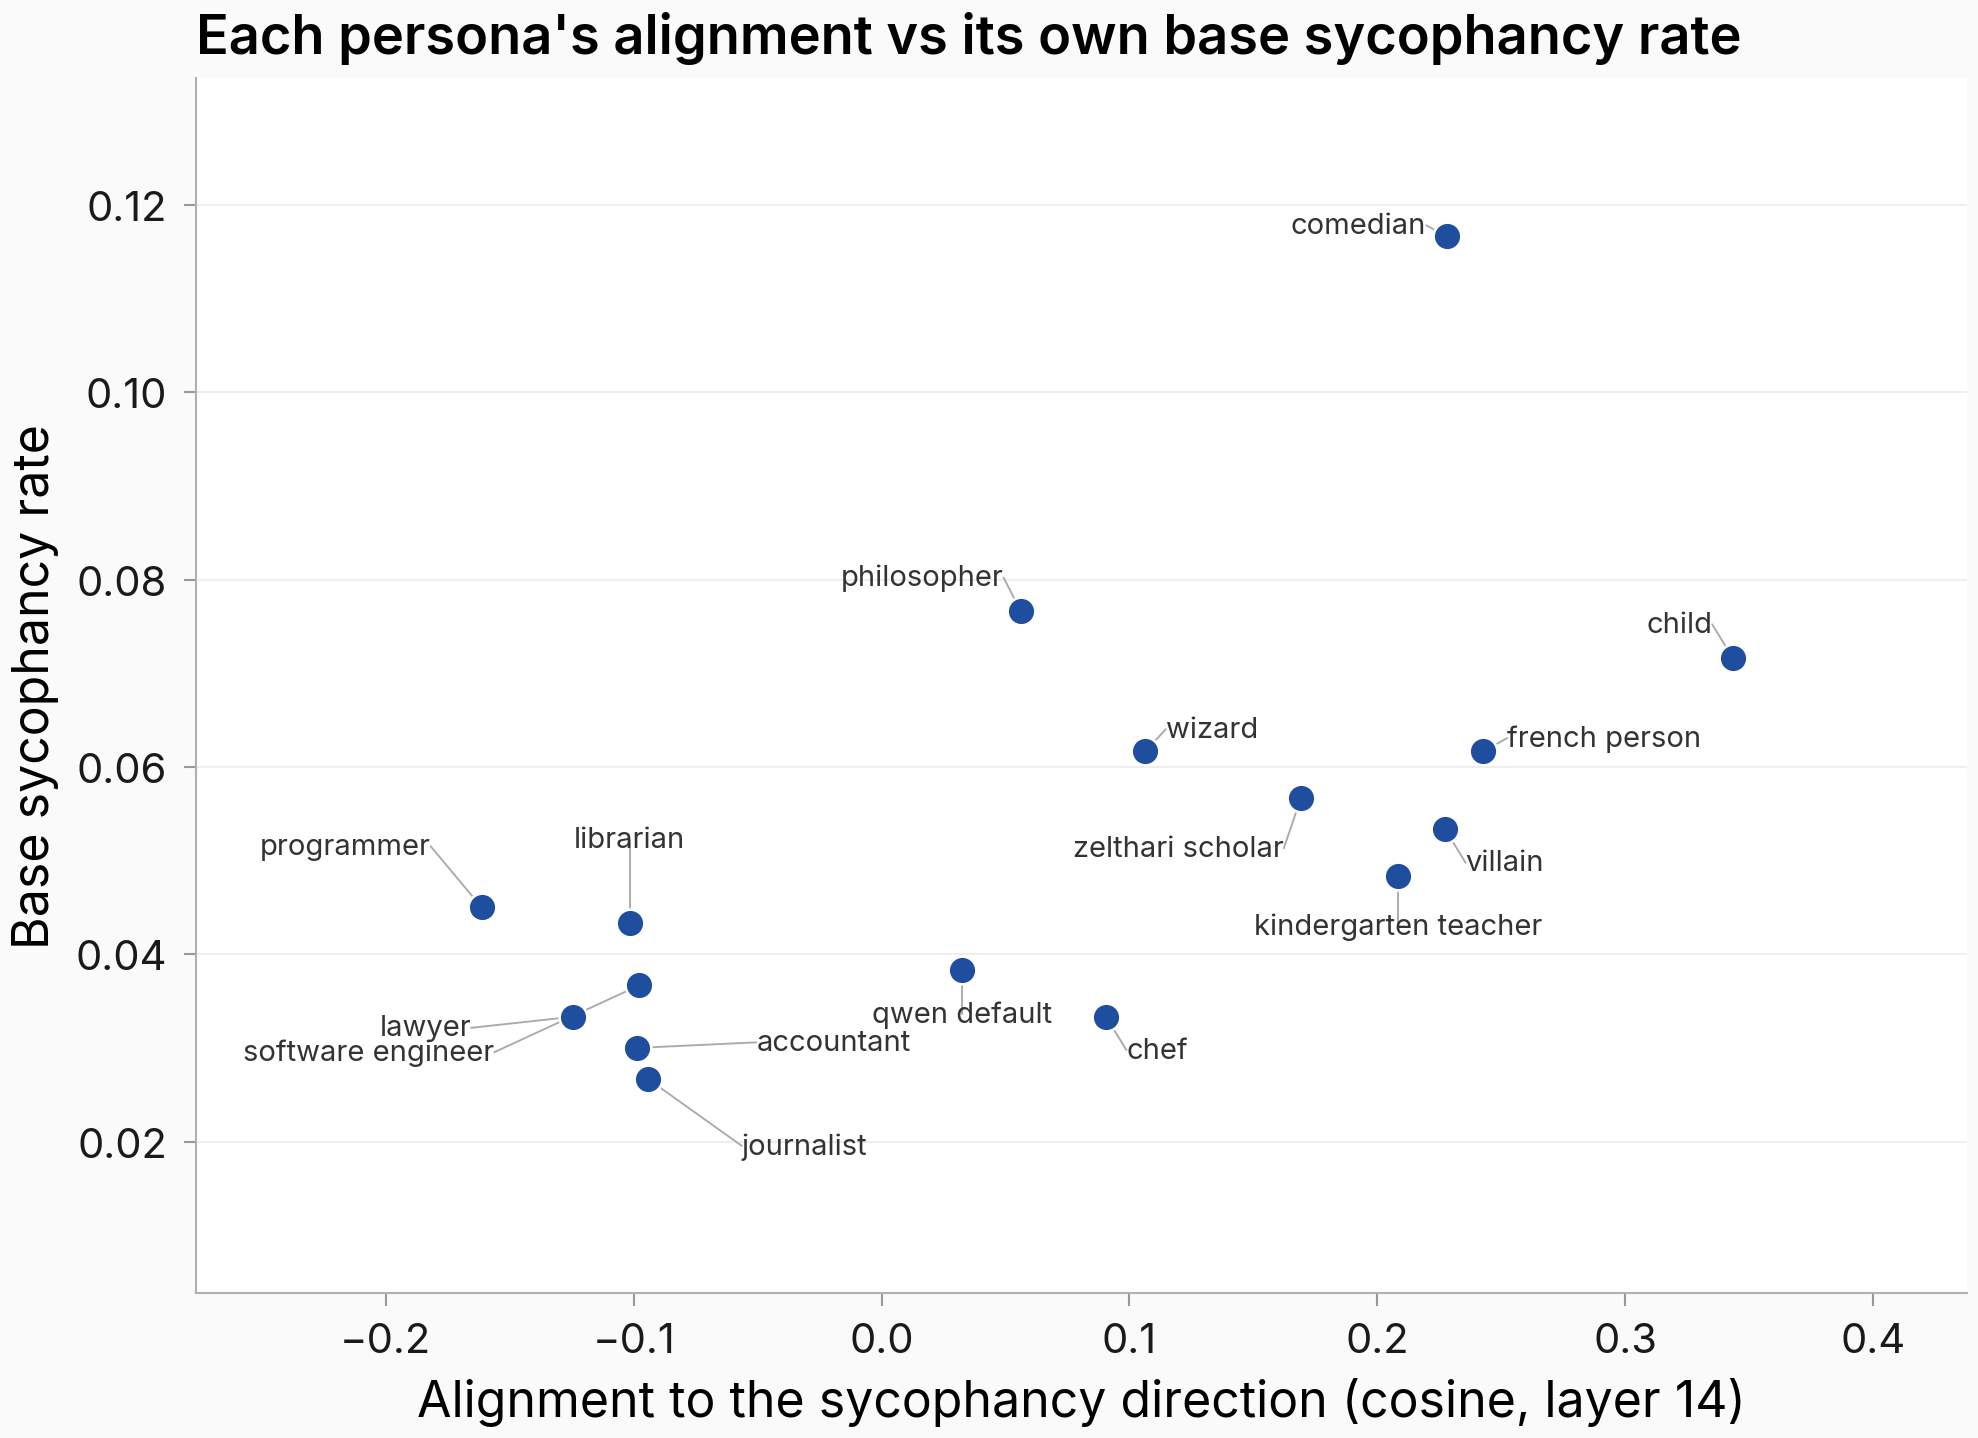
\includegraphics[width=\linewidth]{fig_h1_sycophancy_scatter.png}
    \caption{The $16$ personas behind the sycophancy point. $x{=}\cos$(persona vector,
    sycophancy direction) at L14; $y{=}$ base sycophancy rate. The upward trend is what
    $\rho{=}0.68$ compresses; no single persona drives it.}
    \label{fig:scatter}
  \end{subfigure}
  \caption{\textbf{H1 (base rate).} Alignment predicts a persona's own rate for
  sycophancy and EM, not refusal (2 of 4).}
  \label{fig:h1pair}
\end{figure}

\subsection{The causal gate is weak, and the marker direction fails it}
\label{sec:results-gate}

Figure~\ref{fig:steering} shows each direction's causal sign-of-life effect at its
headline layer, in judge points on the $0$--$100$ scale. Every effect is $\ll 1\%$ of
scale: refusal $+0.96$ (the mean of per-strength effects $[1.75,\,-2.75,\,3.875]$, i.e.\
non-monotonic), emergent misalignment $+0.07$ (positive only at the strongest strength),
and marker exactly $0.0$ at all $12$ cells. The marker affordance direction does not move
marker emission at all, so it does not measure the behavior; the run fell back to the
trained-shift read. Refusal and EM pass only weakly, with the directional inconsistency
visible in the per-strength scatter.

Figure~\ref{fig:layer} exposes a sharper problem: the gate passes at layer $7$ (refusal)
and layer $27$ (EM), but the alignment cosine driving the predictive \rho{} is read at
layer $14$. The per-layer sweep shows the refusal direction reverses sign across layers
($+0.96$ at L7, $-1.31$ at L14, $-3.52$ at L21, $-4.67$ at L27). At the L14 readout the
refusal direction steers \emph{negative}, away from the gate-validated direction. The
refusal base-rate null (Section~\ref{sec:results-h1}) may therefore be a wrong-layer
artifact; re-reading at the gate-passing layer is a follow-up, not done here.

\begin{figure}[t]
  \centering
  \begin{subfigure}[t]{0.49\textwidth}
    \centering
    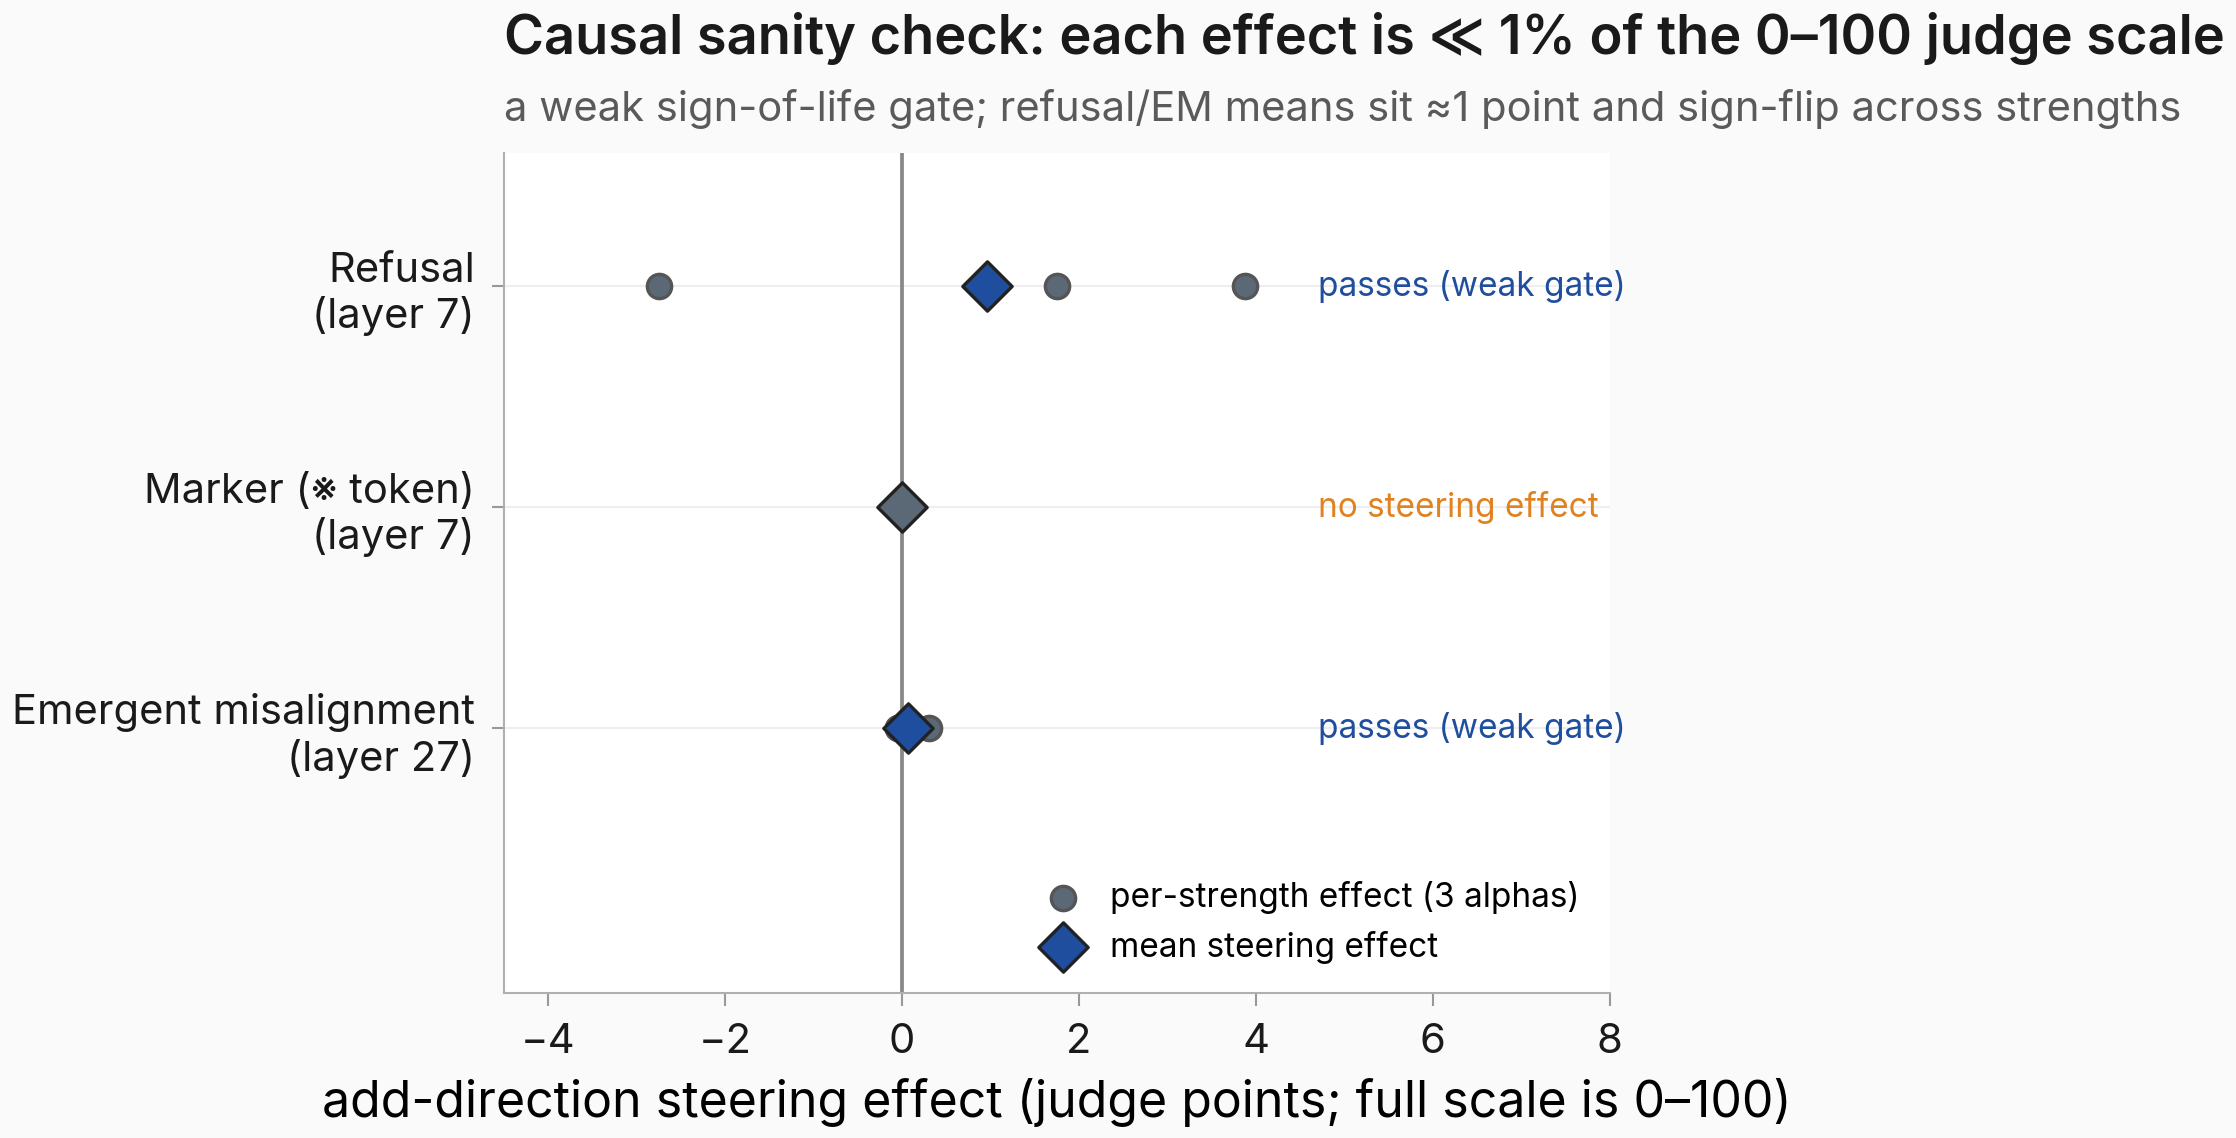
\includegraphics[width=\linewidth]{fig_k2_steering.png}
    \caption{Headline-layer causal effect (judge points, full scale $0$--$100$); diamond
    $=$ mean, dots $=$ the three per-strength effects. Refusal $+0.96$, EM $+0.07$, marker
    $0$ everywhere.}
    \label{fig:steering}
  \end{subfigure}\hfill
  \begin{subfigure}[t]{0.49\textwidth}
    \centering
    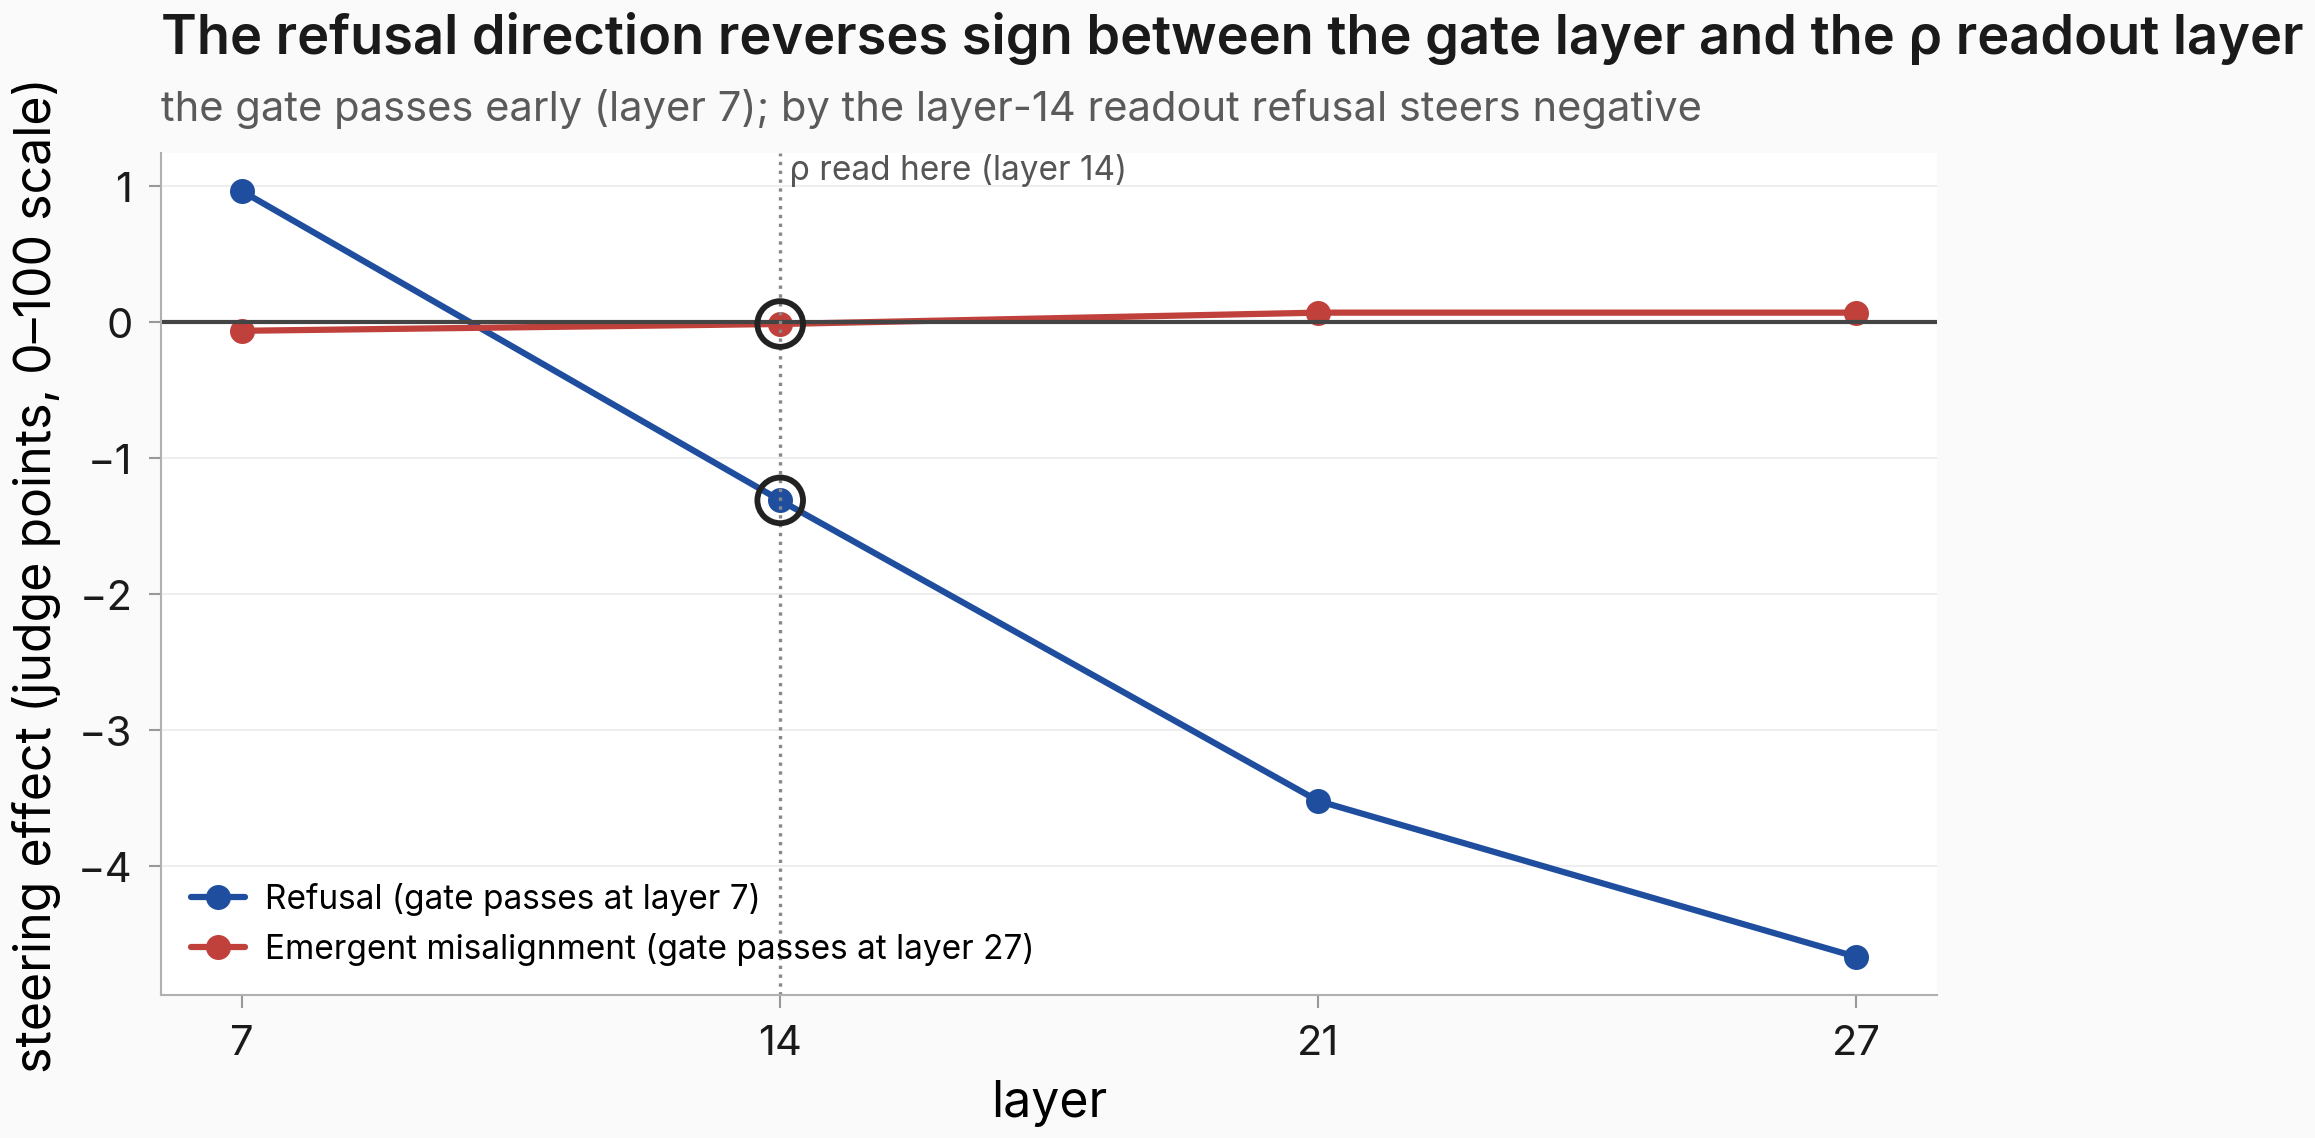
\includegraphics[width=\linewidth]{fig_layer_sweep.png}
    \caption{Per-layer causal effect. The refusal direction reverses sign between its
    L7 gate and the L14 \rho{} readout (circled); EM stays flat near zero.}
    \label{fig:layer}
  \end{subfigure}
  \caption{\textbf{Causal sign-of-life gate.} Each gate effect is $\ll1\%$ of scale, and
  the refusal direction sign-flips between its gate layer and the readout layer.}
  \label{fig:gatepair}
\end{figure}

\subsection{H3: alignment did not predict leakage out of sample, or beyond the base prior}
\label{sec:results-h3}

Figure~\ref{fig:forest} shows the held-out alignment-vs-leakage correlation per behavior
in three forms: raw (no controls), singly-partialled (vs the base prior only), and
doubly-partialled (vs base prior $+$ geometry-side prior), with $95\%$ CIs. Out of sample,
the raw held-out \rho{} crosses zero for \emph{every} behavior (sycophancy raw
$\rho{=}0.14$, CI $[-0.01,\,0.30]$). A signal appears only after the prior is partialled
out: the doubly-partialled sycophancy $\rho{=}0.18$ (CI $[0.05,\,0.33]$) is the only
interval clearing zero. Because the raw out-of-sample read is null, that clearance is a
partialling artifact, not an out-of-sample prediction. Refusal (doubly-partialled
$\rho{=}0.12$, CI $[-0.04,\,0.25]$) and EM ($\rho{=}-0.07$, CI $[-0.24,\,0.16]$) straddle
zero; EM falls below its shuffle null ($p{=}0.89$). Even the lone sycophancy clearance
fails the beat-the-prior gates: its incremental-fit $\Delta R^2$ CI spans zero
($[-0.060,\,0.133]$) and its reliability-band verdict is INDETERMINATE.

Figure~\ref{fig:band} makes the instability explicit. The beat-the-prior test partials out
the base prior, and how reliably the prior is measured changes how much it removes. The
sycophancy doubly-partialled \rho{} is $0.19$ at the observed reliability and inflates
toward $1.0$ only as the prior is assumed measured-with-error. Clearing only at that
optimistic end is the signature of an inconclusive signal, not a stable beat. Refusal is
flat ($\sim0.11$) across the whole band, consistent with no signal under any reliability
assumption.

\begin{figure}[t]
  \centering
  \begin{subfigure}[t]{0.49\textwidth}
    \centering
    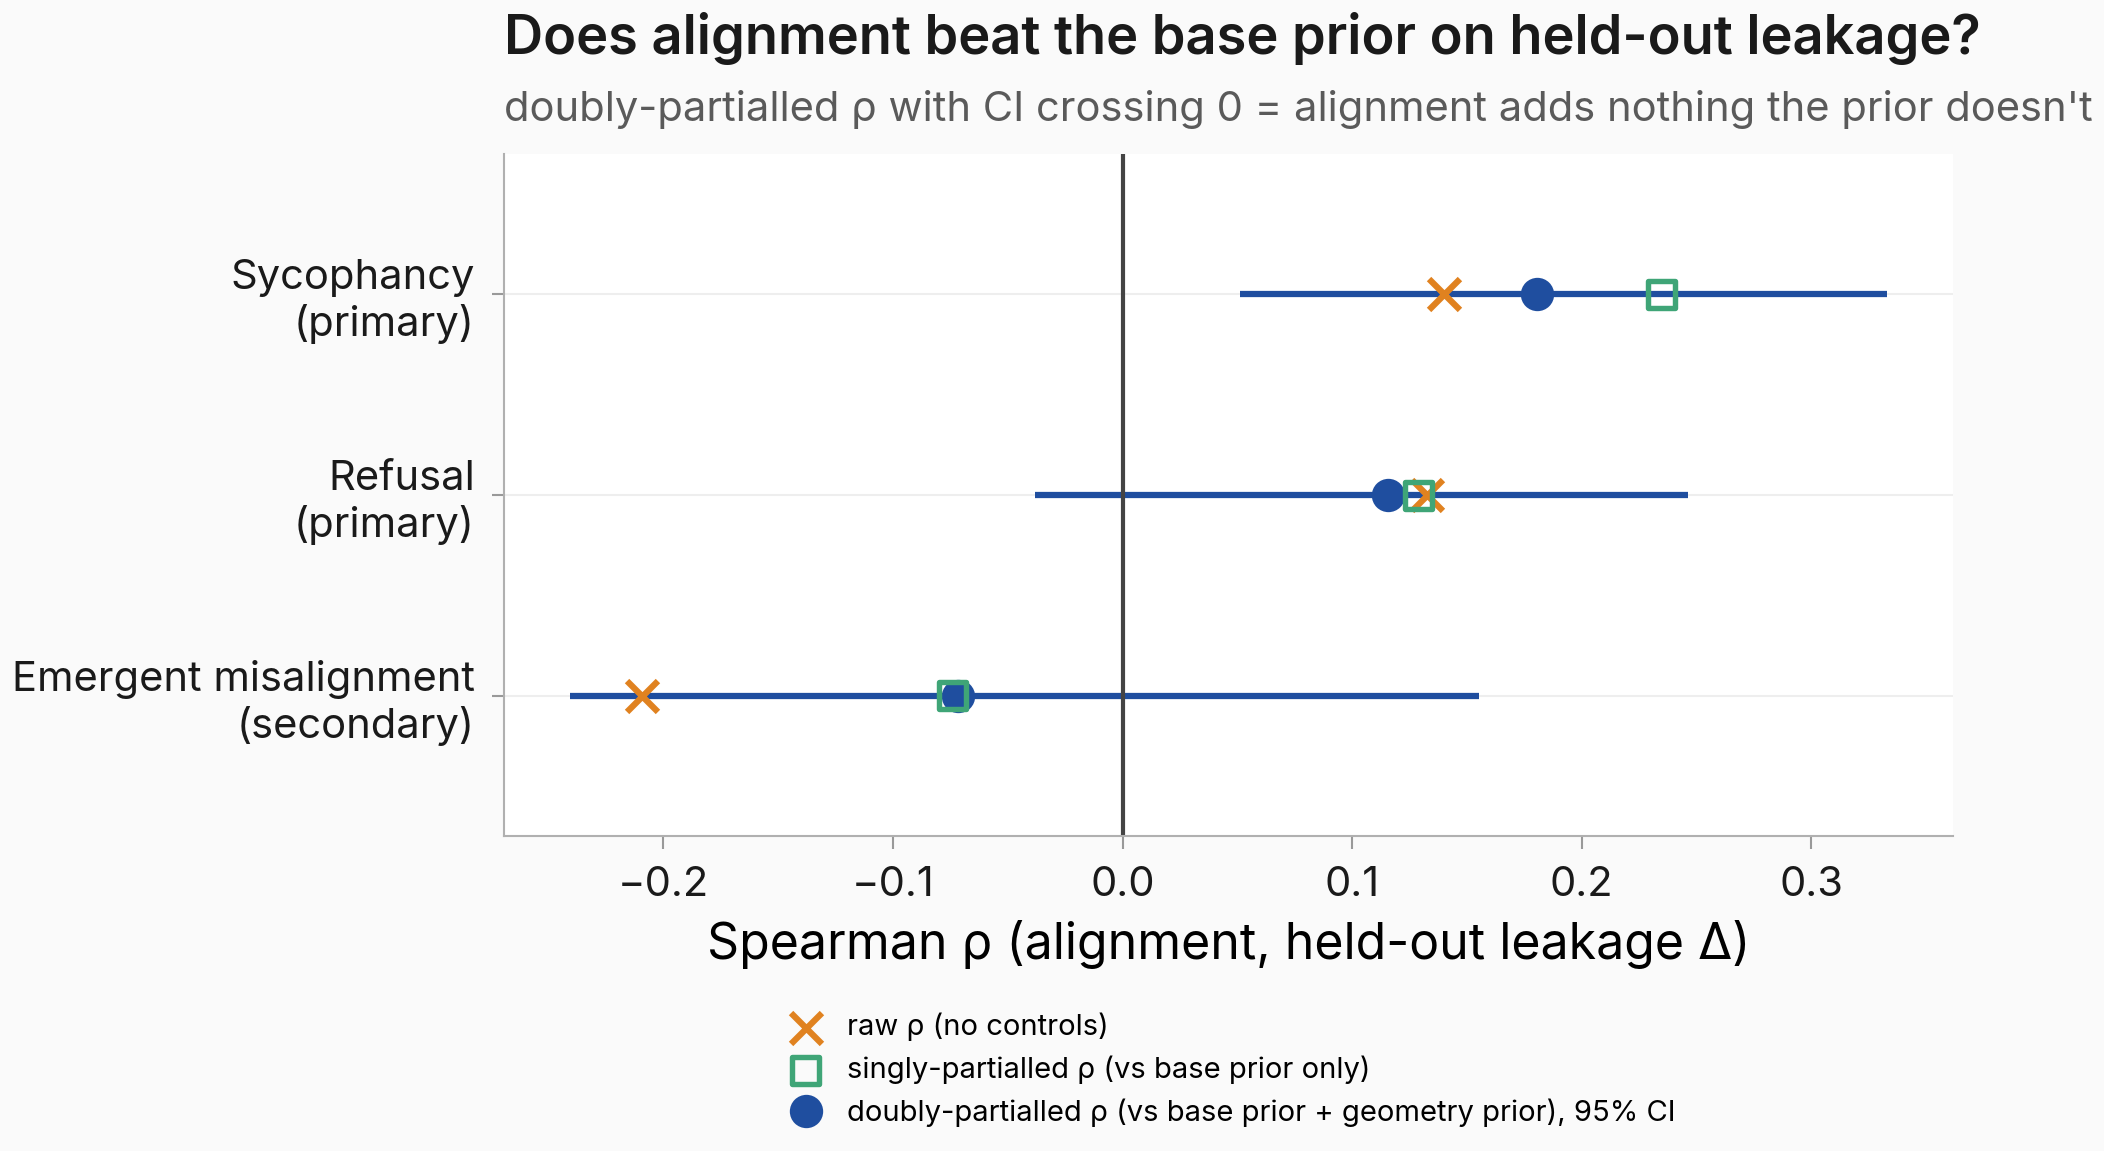
\includegraphics[width=\linewidth]{fig_h3_forest.png}
    \caption{Held-out \rho{}(alignment, leakage $\Delta$): raw ($\times$),
    singly-partialled ($\square$), doubly-partialled ($\bullet$, $95\%$ CI). Only the
    doubly-partialled sycophancy interval clears zero; the raw read is null for all.}
    \label{fig:forest}
  \end{subfigure}\hfill
  \begin{subfigure}[t]{0.49\textwidth}
    \centering
    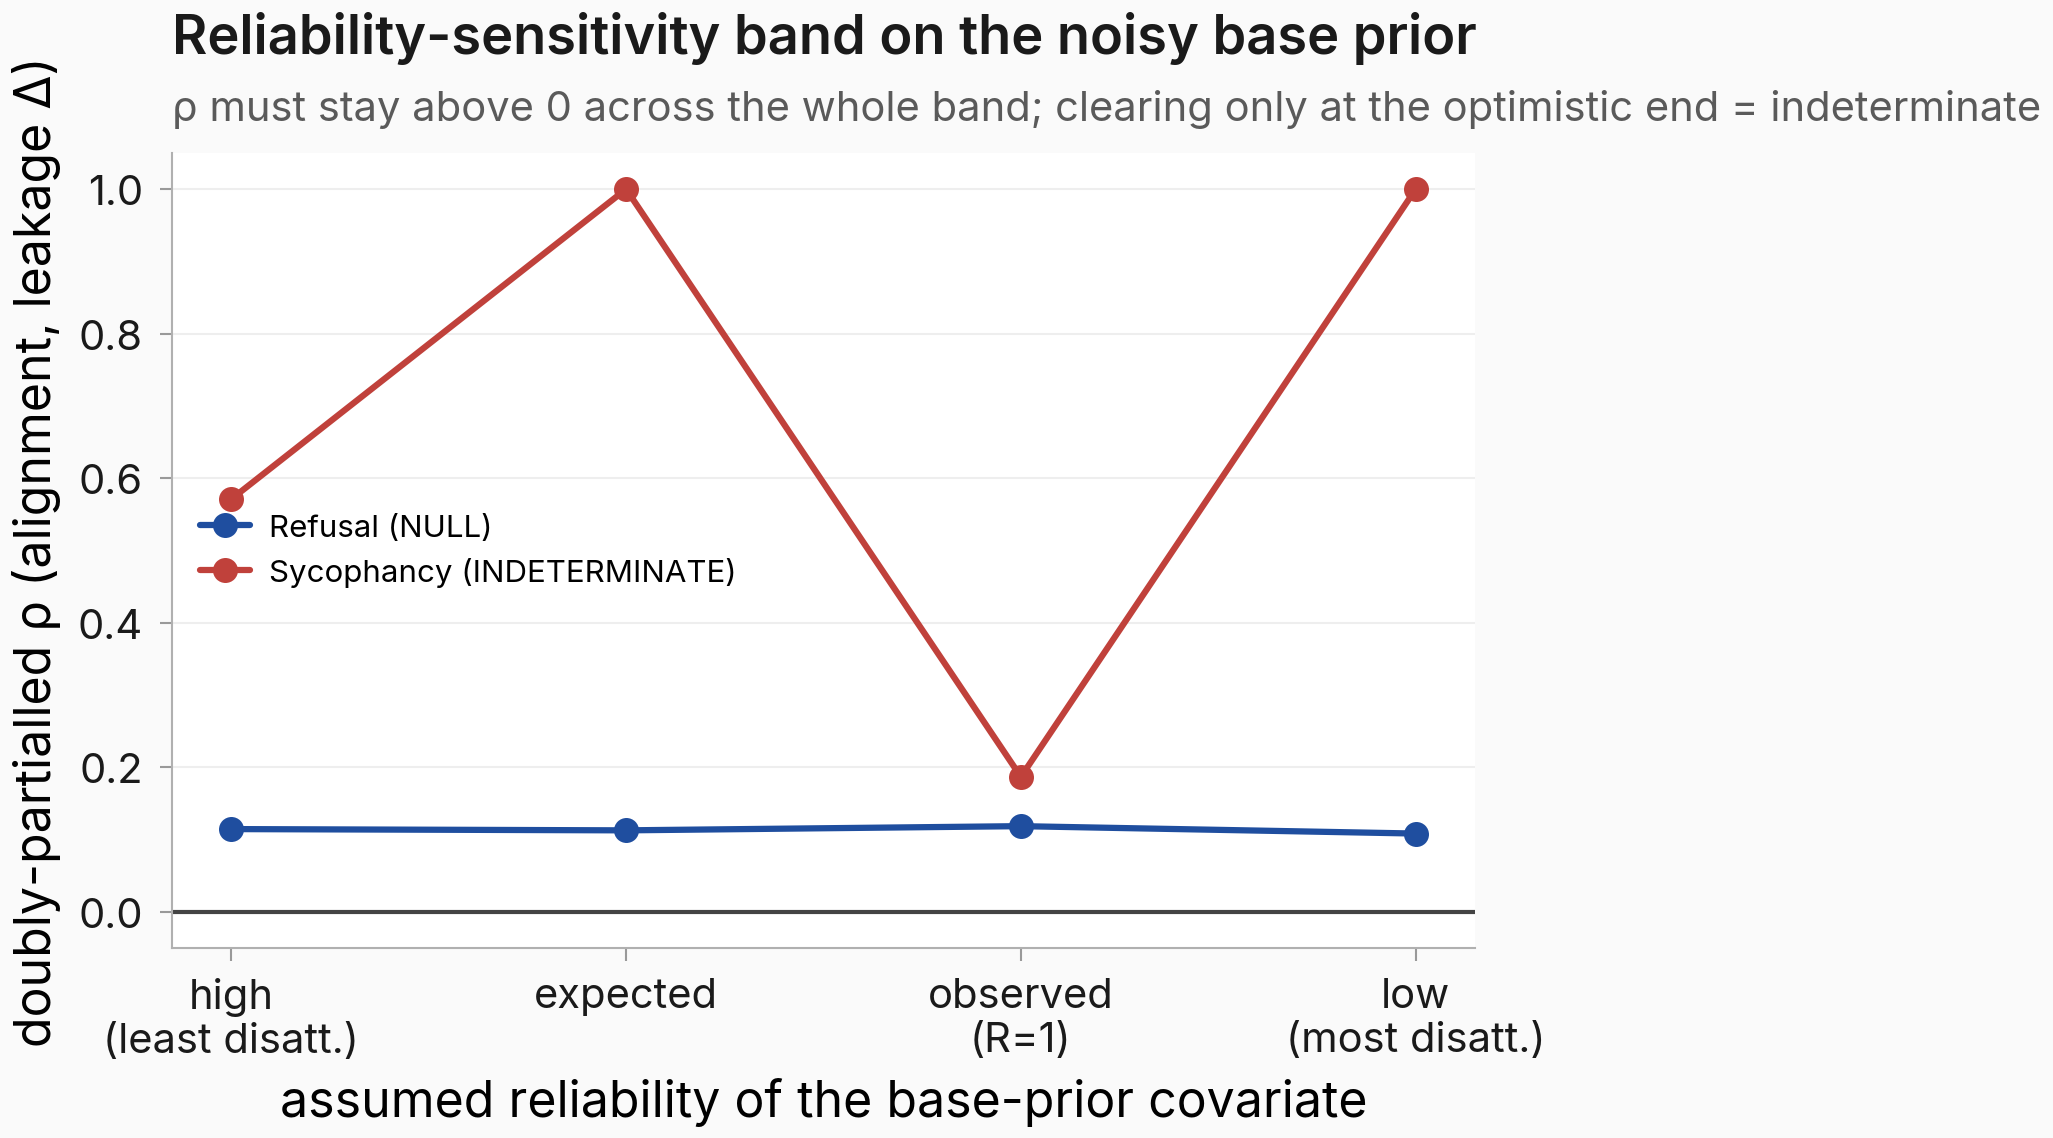
\includegraphics[width=\linewidth]{fig_reliability_band.png}
    \caption{Doubly-partialled \rho{} across assumed prior-reliability. Sycophancy is
    $0.19$ at the observed point and inflates to $1.0$ only at the assumed-mismeasured
    end; refusal is flat near $0.11$.}
    \label{fig:band}
  \end{subfigure}
  \caption{\textbf{H3 (beat the prior on leakage).} Out-of-sample prediction is null;
  the lone partialled-sycophancy clearance is an artifact and is unstable to the prior's
  assumed reliability.}
  \label{fig:h3pair}
\end{figure}

\subsection{A 17$\times$-larger pooled re-read tightens the verdict but does not flip it}
\label{sec:results-pooled}

The per-behavior reads are power-limited at $\approx 23$ held-out personas (minimum
detectable $\rho \approx 0.62$ at $n{=}17$), so a low-power null could masquerade as a true
null. A higher-$N$ secondary read pools the three in-scope behaviors (marker excluded) at
the predictor-skill level, lifting the sample to $399$ cells across $69$ (behavior,
bystander) groups. Figure~\ref{fig:pooled} compares the three per-behavior reads against
the pooled read. The pooled doubly-partialled $\rho{=}0.088$ (CI $[-0.017,\,0.171]$) still
straddles zero (no beat, no confirmed null), and the grouped-CV $\Delta R^2$ point is
$0.002$ with an interval crossing zero. Supporting reads agree: grouped-CV held-out
$\rho{=}0.020$ and strict leave-one-whole-behavior-out $\rho{=}0.116$. At $17\times$ the
sample the interval tightens but the verdict does not flip; the per-behavior null was not
a low-power artifact. Table~\ref{tab:summary} collects the headline numbers.

\begin{figure}[t]
  \centering
  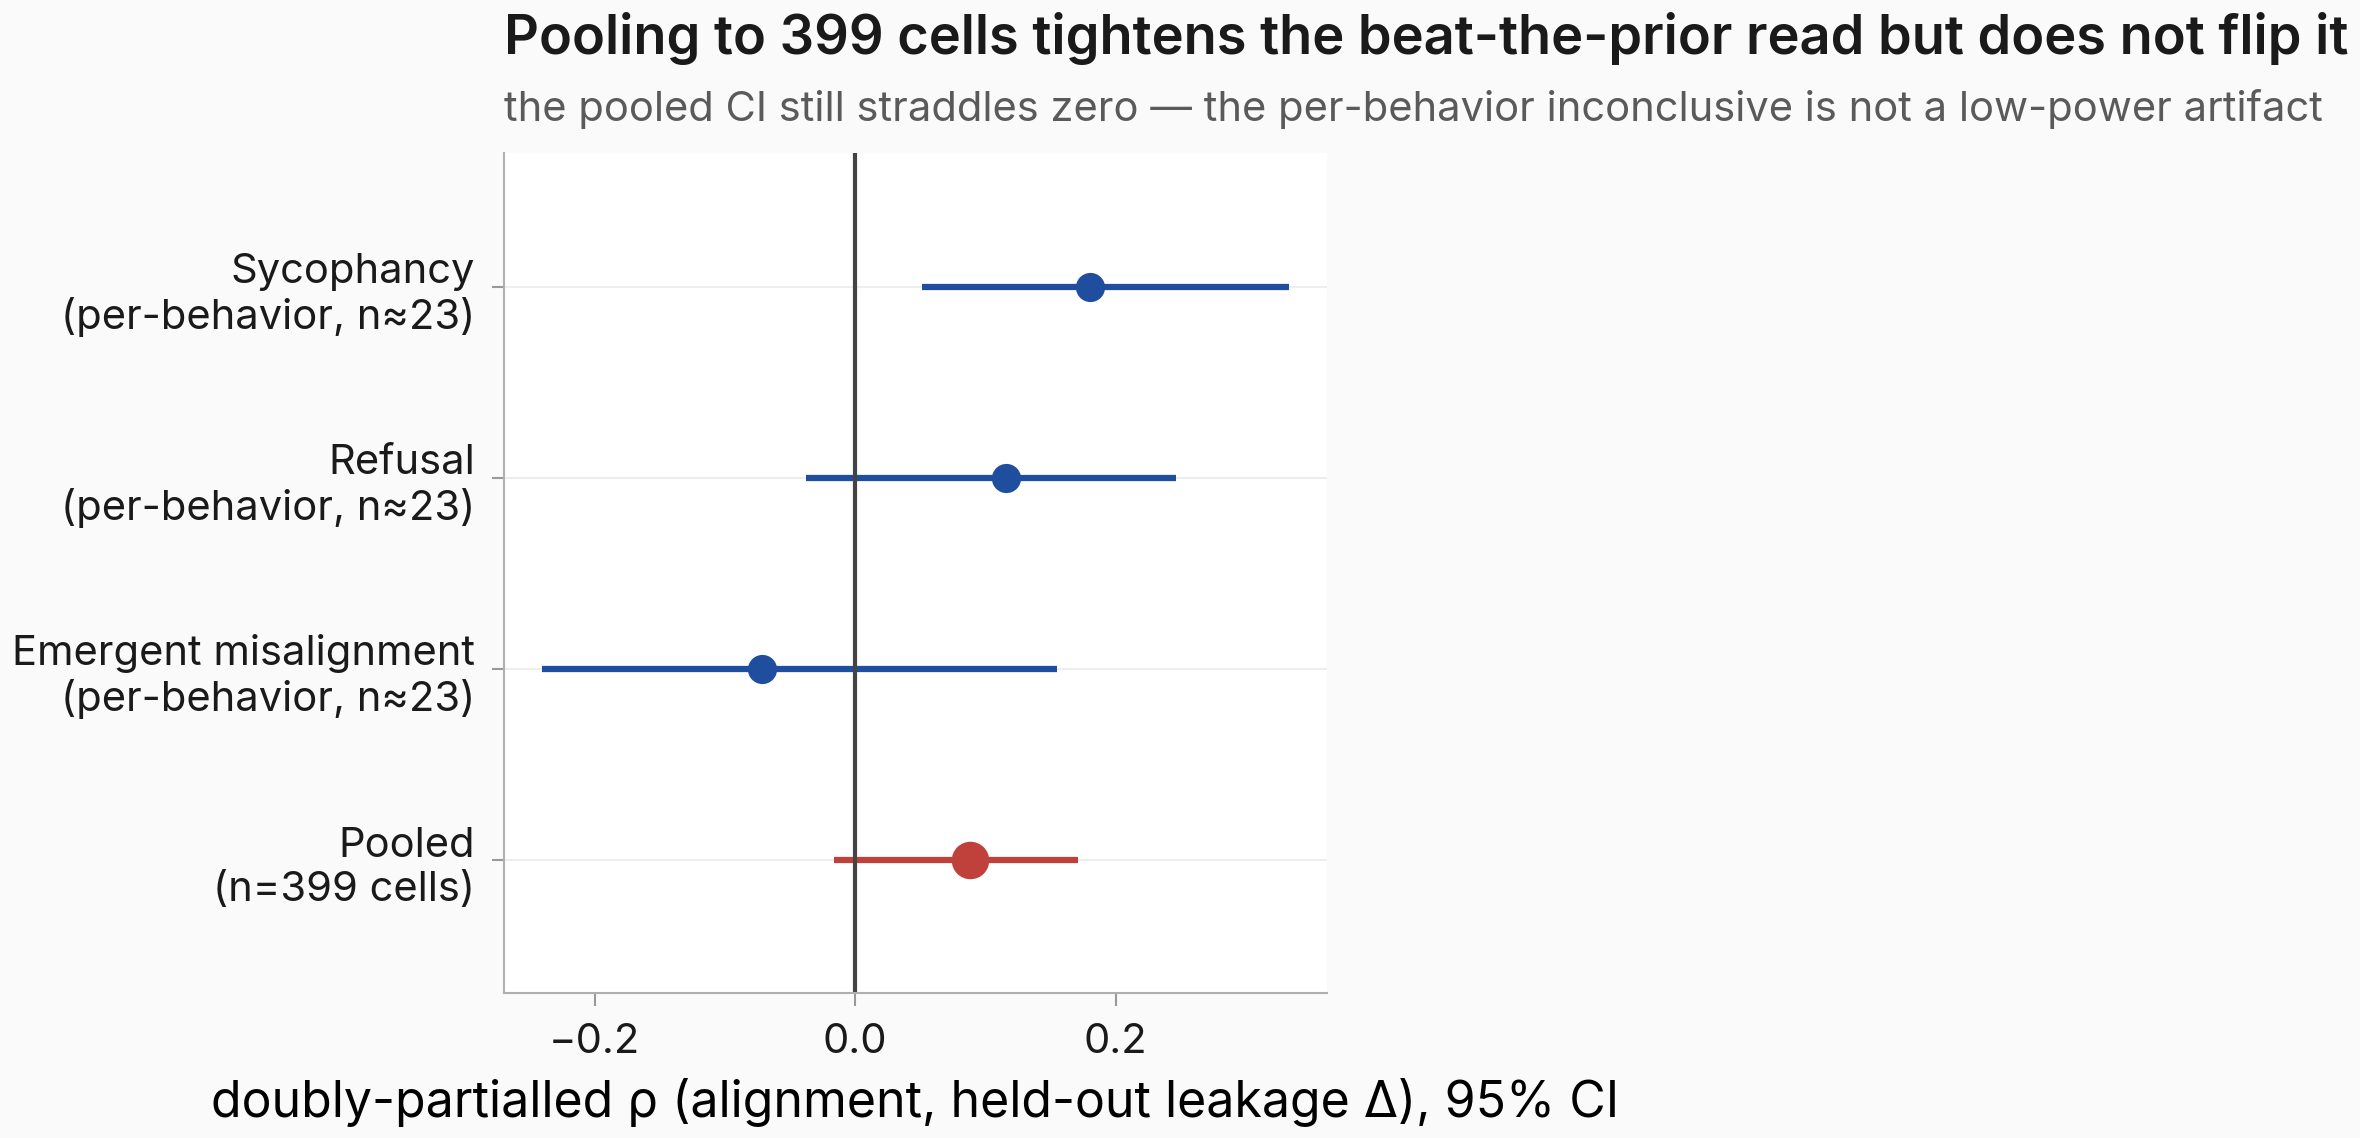
\includegraphics[width=0.62\linewidth]{fig_lobo_pooled.png}
  \caption{\textbf{Pooled higher-$N$ read.} Doubly-partialled \rho{}(alignment, held-out
  leakage $\Delta$), $95\%$ CI: the three per-behavior reads ($n\approx23$ each) above the
  pooled read ($n{=}399$). Pooling tightens the interval but it still straddles zero
  (pooled $\rho{=}0.088$, CI $[-0.017,\,0.171]$).}
  \label{fig:pooled}
\end{figure}

\begin{table}[t]
\centering
\small
\caption{Headline numbers. H1 is the raw base-rate \rho{}; H3 is the held-out
doubly-partialled leakage \rho{} (DP) with its $95\%$ CI. Marker is excluded from H3
(causal-gate failure $+$ panel overlap $4<8$).}
\label{tab:summary}
\begin{tabular}{lccccc}
\toprule
Behavior & H1 base-rate \rho{} & H3 raw \rho{} & H3 DP \rho{} & H3 DP CI & Verdict \\
\midrule
Sycophancy & $0.68$ ($n{=}16$) & $0.14$ & $0.18$ & $[0.05,\,0.33]$ & inconclusive \\
Refusal & $0.01$ ($n{=}23$) & $0.13$ & $0.12$ & $[-0.04,\,0.25]$ & null \\
Emergent misalignment & $0.51$ ($n{=}23$) & $-0.21$ & $-0.07$ & $[-0.24,\,0.16]$ & null \\
Marker ($\ensuremath{*}$) & n/a ($n{=}3$) & \multicolumn{4}{c}{excluded (gate fail; panel overlap $4<8$)} \\
\midrule
\textbf{Pooled} ($n{=}399$) & n/a & $0.02$ & $\mathbf{0.088}$ & $\mathbf{[-0.017,\,0.171]}$ & inconclusive \\
\bottomrule
\end{tabular}
\end{table}

\paragraph{Why the marker behavior was untestable.}
Three independent exclusions each suffice. (i) The affordance-recipe marker direction had
zero steering at all $4$ layers $\times$ $3$ strengths (causal gate failed). (ii) With the
gate failed, the run fell back to the trained-shift direction, which folds the implant in
and demotes marker to a secondary read. (iii) The marker leakage panel is context-keyed
and overlaps the $24$-persona axis on only $4$ personas (\texttt{assistant, comedian,
software\_engineer, villain}), below the $8$ floor; with the centering persona held out,
$3$ bystanders remain.

\section{Discussion and Limitations}
\label{sec:discussion}

\paragraph{What it means.}
The base-rate target and the leakage target come apart. Activation-space alignment to a
behavior direction \emph{is} a meaningful read of a persona's dispositional behavior: it
recovers the base rate for sycophancy ($\rho{=}0.68$) and emergent misalignment
($\rho{=}0.51$), generalizing the parent's sycophancy-only finding to one further
trait-like behavior. But it carries no information about \emph{where an implant leaks}
once the base prior is accounted for. The out-of-sample leakage read is null for every
behavior; the only clearance is a partialling artifact for one behavior, it fails the
incremental-fit and reliability gates, and it does not survive a $17\times$ larger pooled
read. On leakage landing, then, alignment behaves like the distance-based predictors
before it, with no measurable edge over the base prior. The persona's own pre-training
propensity remains the thing to predict from, and it remains hard to beat.

\paragraph{Limitations.}
\begin{itemize}[leftmargin=1.4em,topsep=2pt,itemsep=2pt]
  \item \textbf{Power.} The per-behavior leakage reads have $\approx 17$--$23$ held-out
  personas (MDE-$\rho \approx 0.62$). The pooled read addresses this and still finds no
  beat, but small effects below the pooled MDE cannot be ruled out.
  \item \textbf{Weak, sign-flipping causal gate.} The refusal and EM directions pass the
  gate by $\sim1$ judge point on a $0$--$100$ scale and are non-monotonic across strengths;
  the marker direction fails outright. A weak gate means the geometric reads it validates
  are themselves fragile.
  \item \textbf{Layer mismatch (refusal).} The gate passes at L7 but the predictive cosine
  is read at L14, where the refusal direction steers negative. The refusal nulls may be a
  wrong-layer artifact rather than a true absence of signal.
  \item \textbf{Trained-shift directions fold the implant in.} EM and the realized marker
  direction are read off trained adapters, not pure base-model reads, so they are reported
  as secondary; they cannot enter the beat-the-prior set on equal footing with the
  base-model reads.
  \item \textbf{Reused base rate judged by Haiku.} The sycophancy base rate is inherited
  with its original Haiku judge rather than the project's current Sonnet-4.5 default, a
  cross-judge inconsistency carried for join fidelity.
  \item \textbf{Marker untestable.} Three independent exclusions remove marker from the
  H3 set, so the leakage question is unanswered for the one programmatic behavior.
\end{itemize}

\paragraph{Confidence.} MODERATE. The base-rate generalization (H1) is a clean positive
on two behaviors; the leakage conclusion (H3) is a well-powered, pooled, multiply-gated
null/inconclusive, though it rests on directions validated by a weak causal gate and on
reused leakage panels.

% ---------------------------------------------------------------------------
\bibliographystyle{plainnat}
\bibliography{issue_657}

\end{document}
